\documentclass[conference]{IEEEtran}

%\usepackage{cite}
\usepackage{ngerman}
\usepackage[utf8]{inputenc}
\usepackage[T1]{fontenc}
\usepackage{listings}
\usepackage{makecell}
%\usepackage[section]{placeins}


  \usepackage[pdftex]{graphicx}
  \graphicspath{{images/}}
%   \DeclareGraphicsExtensions{.pdf,.jpeg,.png}


\hyphenation{op-tical net-works semi-conduc-tor}


\begin{document}

\title{%
  Entwicklung domänenspezifischer Sprachen mit ANTLR am Beispiel eines Pac-Man-Klons\bigbreak
  \large Studiengang Medieninformatik Master\\Beuth Hochschule für Technik Berlin}


\author{\IEEEauthorblockN{Marcel Brüning}
\IEEEauthorblockA{
s67176@beuth-hochschule.de}
\and
\IEEEauthorblockN{Simon Lischka}
\IEEEauthorblockA{simon@lischka.co}
\and
\IEEEauthorblockN{Marcel Piater}
\IEEEauthorblockA{s67357@beuth-hochschule.de}}

\maketitle

\lstset{%
  basicstyle=\footnotesize\ttfamily
  }
\begin{abstract}
Die folgenden Seiten beschreiben die Entwicklung eines Pac-Man Browserspiels mit JavaScript. Die Schwerpunkte des Projekts liegen in der automatischen Codegenerierung mit domänenspezifischen Sprachen (DSL) für die Levels und die artifizielle Intelligenz (AI). Die DSL der AI definiert verschiedene Strategien der vom  Computer gesteuerten Spielfiguren.
\end{abstract}

\IEEEpeerreviewmaketitle



\section{Über das Spiel}

Der Inhalt dieses Absatzes ist das Spielprinzip von Pac-Man und die Entwicklung der Spiellogik. Dabei werden die eingesetzten Technologien beschrieben.

\subsection{Spielprinzip}

Pac-Man ist eine Spielfigur, die durch ein Labyrinth so effektiv wie möglich gesteuert werden soll, um alle vorhandenen Punkte zu sammeln. Bewegliche Gegner (vier Geister), die vom Computer gesteuert werden, sowie ein komplexes Labyrinth erschweren den Siegeszug. Pro Spiel verfügt Pac-Man über drei Leben. Wird er von einem Gegner gefasst, so geht ein Leben verloren. In dem Labyrinth gibt es durch das Sammeln von Münzen die Möglichkeit, die Gesamtpunktzahl zu erhöhen.

Über Früchte in den Ecken des Spielfelds gelangt Pac-Man in den Angriffsmodus. Er wird für kurze Zeit vom Gejagten zum Jäger und kann seinerseits Geister fressen. Das verhilft ihm zu zusätzlichen Punkten. Schafft es Pac-Man innerhalb der drei Leben sämtliche Punkte auf dem Spielfeld zu konsumieren, so hat er das Level erfolgreich absolviert und startet ein neues Level.


\subsection{Verwendete Technologien}
Das Spiel ist in JavaScript implementiert. Teile des Codes werden mit dem Parser-Generator \texttt{ANTLR4} auf Basis der DSL erzeugt. Dieser Code wird von der Applikation angesteuert.

Ein naheliegender Gedanke in der Planungsphase war es, die JavaScript-Implementierung von \texttt{ANTLR4} zu verwenden. Auf diese Weise ließe sich eine einheitliche Programmiersprache in der gesamten Codebasis einsetzen. Ein programmiertechnischer Austausch zwischen allen Teammitgliedern könnte dadurch erleichtert werden. Dieser Austausch kann aus Code-Reviews und dem Klären von sprachspezifischen Problemen bestehen.

Da die Java-Implementierung von \texttt{ANTLR4} etablierter erscheint und über ausführlichere Dokumentation verfügt als die JavaScript-Variante, haben wir von der Verwendung von \texttt{ANTLR4} für JavaScript abgesehen. Wir hatten die Vermutung, dass die zusätzliche Einarbeitungszeit und für uns unerwartetes Verhalten der JavaScript-Implementierung den zeitlichen Rahmen des Projektes übersteigen würde.

Wir haben jedoch für die JavaScript-Codebasis gezielt Technologien zur Qualitätssteigerung ausgewählt. Hierzu gehört das Framework \texttt{RequireJS}, welches die Modularisierung und das Importieren von Klassen ähnlich wie in Java ermöglicht. Von \texttt{ANTLR4} erzeugte JavaScript-Klassen müssen als Module ladbar sein. \texttt{RequireJS} war für uns deshalb Voraussetzung um unser  Vorhaben erfolgreich umsetzen zu können.

Objektorientiertes Programmieren nach dem Paradigma \emph{Separation of Concerns} (SoC) und der Aufbau einer übersichtlichen Projektstruktur werden durch Trennung von Klassen in einzelne Dateien durch \texttt{RequireJS} ebenfalls stark erleichtert.

\texttt{Underscore.js} bietet eine Reihe von Helferfunktionen, die darauf ausgerichtet sind, funktionale Programmierung zu erleichtern\footnote[1]{Underscore.js Einführung, http://underscorejs.org/}. Mit \texttt{Underscore.js} sind häufig eingesetzte Idiome wie Listeniterationenin in kürzerer Syntax und auf höherem Abstraktionsgrad als durch native JavaScript-Sprachmittel abbildbar. Hierdurch ergibt sich weniger Raum für Fehler.

Kritische Funktionen wurden in JavaScript mit \texttt{Jasmine}-Unit Tests versehen. Eine hohe Testabdeckung, wie sie mit Test Driven Development möglich ist, haben wir jedoch nicht priorisiert.

\subsection{Umsetzung}
\label{umsetz}
Das zu spielende Level besteht aus einem 2-dimensionalem Array. Die Elementes des Spielfelds sind durch Zahlencodes abgebildet. Eine Null steht dabei für ein freies Stück Weg. Codes Eins und Zwei stehen für ein begehbares Feld mit einem Punkt oder einer Frucht. Wände werden durch Code Drei repräsentiert und sind von Pac-Man und den Gegnern nicht begehbar.

Zur Darstellung laden wir Bildobjekte und zeichen sie auf einem Canvas-Element des HTML Dokuments. Zum Darstellen der Bildobjekte wird durch das Array iteriert und für jedes Array-Element ein dem Zahlencode zugehörige Bildobjekt auf den 2D-Kontext des Canvas gezeichnet.

Ein zweites Canvas-Element stellt Spielfiguren dar. Es ist transparent über dem Canvas-Element des Levels positioniert. Die Motivation hierfür ist, dass der Zustand der Spielfiguren sich in der Regel häufiger ändert als der des Spielfeldes. Ein Flackern, was durch zusätzliches Neuzeichnen des Levels bei jeder Figurveränderung entstehen kann, wird durch Trennung in zwei Canvas-Elemente reduziert.

Die Figuren operieren auf dem selben Koordinatensystem wie das Level. Abbildung \ref{pac_screen} zeigt das ausgeführte Spiel.

\begin{figure}[!t]
\centering
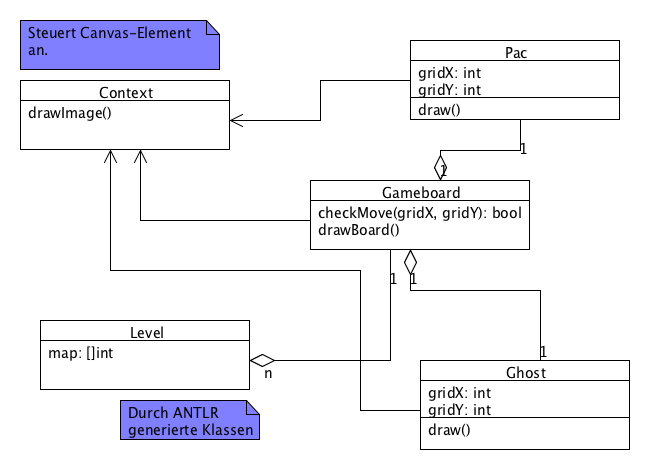
\includegraphics[width=3.3in]{gameboard_and_figures.png}

\caption{Reduziertes Klassendiagramm der zentralen Spielklassen}
\label{main_classes}
\end{figure}

Das Klassendiagramm in Abbildung \ref{main_classes} stellt die beteiligten JavaScript-Objekte dar. Die Objekte von Spieler und Gegner (Pac und Ghost) führen die Instanzvariablen gridX und gridY, die Koordinaten des Levels sind. Die Funktion checkMove() der Klasse Gameboard gleicht den nächsten Schritt einer Figur mit dem Array des Levels ab. Bei Zahlencode Null, Eins oder Zwei liefert sie \texttt{true} zurück und erlaubt den gewünschten Schritt der Figur. Entsprechend wird bei einer Drei, also einer Wand \texttt{false} zurückgeliefert und verhindert somit den nächsten Schritt der Spielfigur. Diese Funktion wird von Klassen Ghost und Pac bei der Umsetzung des nächsten Spielzugs verwendet.

Um die Bewegungen der Figuren sichtbar zu machen, existiert die Funktion updateOnInterval(), die durch den Scheduler des Browsers alle 150 Millisekunden aufgerufen wird. Sie zeichnet das Level und die Spielfiguren nach vorgenommener Aktualisierung neu. In der Methode werden Kollisionsabfragen der Klasse GameBoard aufgerufen, die prüfen ob Pac-Man gerade einen Punkt bzw. eine Frucht frisst (Methode \texttt{checkPacsEating()}) oder mit einem Geist kollidiert (Methode \texttt{checkKills()}). Die im Spiel agierende AI berechnet in jedem Interval die Richtung der Geister neu. Ihre Berechnung bezieht sich also immer genau auf einen Spielzug.

\begin{figure}[!t]
\centering
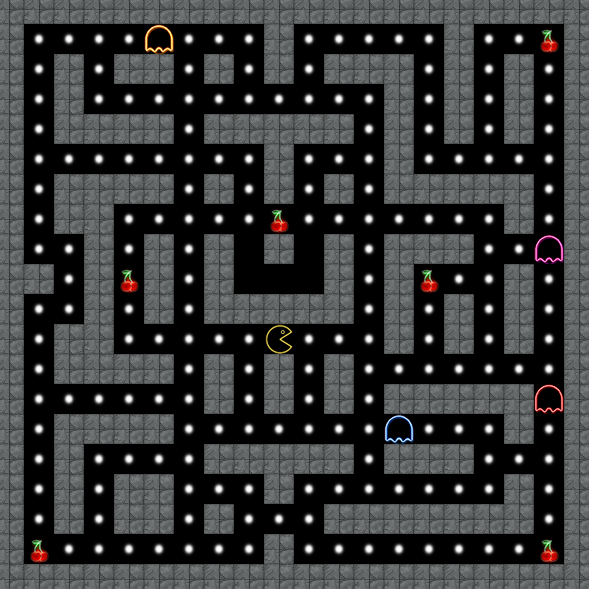
\includegraphics[width=2.9in]{screenshot.png}

\caption{Screenshot des ausgeführten Pac-Man Spiels.}
\label{pac_screen}
\end{figure}

Abbildung \ref{fmc_tam} stellt das FMC-TAM Diagramm des Spiels dar. Ghost und Pac-Man sind als Akteure dargestellt, die ihre Position in Abstimmung mit dem Ergebnis von \texttt{checkMove()} aktualisieren. Akteur Strategy und Speicher Level werden durch \texttt{ANTLR4} generiert. Im Zusammenhang mit Strategy ist Mittler GhostQuery relevant. GhostQuery stellt die Schnittstelle des generierten Codes zum Spiel dar und wird bei der Beschreibung der AI DSL in Abschnitt \ref{ai_dsl} näher erläutert.

\begin{figure}[!t]
\centering
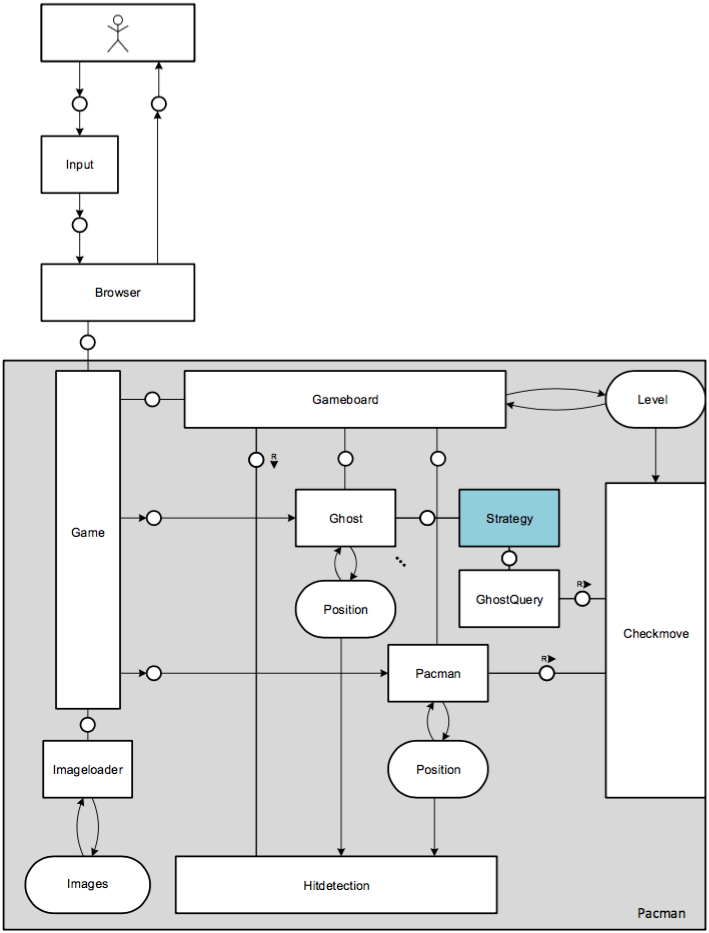
\includegraphics[width=3.0in]{tam.png}

\caption{FMC-TAM Diagramm der umgesetzen Applikation}
\label{fmc_tam}
\end{figure}

Interessant ist, dass die Akteure sich nicht auf eine einheitliche Modularisierungseinheit, also Beispielsweise nur Klassen abbilden. \texttt{Checkmove} wird im vorliegenden Entwicklungsstand durch eine einzelne Methode repräsentiert, Hitdetection durch mehrere Methoden der Klasse Gameboard. Akteure \texttt{Pac-Man} und \texttt{Ghost} existieren als eigene Klassen, ebenso wie \texttt{Strategy} und \texttt{GhostQuery}.

Es ist wahrscheinlich, dass eine Auslagerung von Hitdetection in eine eigenständige Klasse bei zunehmender Komplexität sinnvoll wäre und dadurch das Design durch die Einhaltung des SoC-Paradigmas verbessert werden würde. Durch die Aufstellung des FMC-TAM Diagramms lässt sich diese bevorstehende Designänderung antizipieren, auch wenn wir uns in der vorliegenden Implementierung dazu entschlossen haben, sie nicht umzusetzen.

\section{Codegenerierung}
\texttt{ANTLR4} generiert auf Grundlage der DSL Lexer zur lexikalischen Analyse und Parser zur syntaktischen Analyse.
Wir haben uns bei der Umsetzung der Level- und der AI DSL für  das Einsetzen von Listener Klassen zum Traversieren des Abstrakten Syntaxbaums (AST) entschlossen.

Für beide Grammatiken erstellten wir Subklassen der generierten Listener. Diese Klassen enthalten jeweils eine Datenstruktur als Instanzvariable, die beim Traversieren des AST befüllt wird. Im Fall der Level DSL handelt es sich um eine Liste und bei der AI DSL um eine Baumstruktur.

Erst nach Beenden der Traversierung werden die Daten in der Klasse \texttt{CodeGenerator} durch Interpretation der Datenstrukturen, die in den Listenern erzeugt wurden, geschrieben. Abbildung \ref{antlr_classes} stellt die beteiligten Klassen dar. Bei \texttt{totalValues} und \texttt{initialRoot} handelt es sich um diese Datenstrukturen.

\begin{figure}[!htb]
\centering
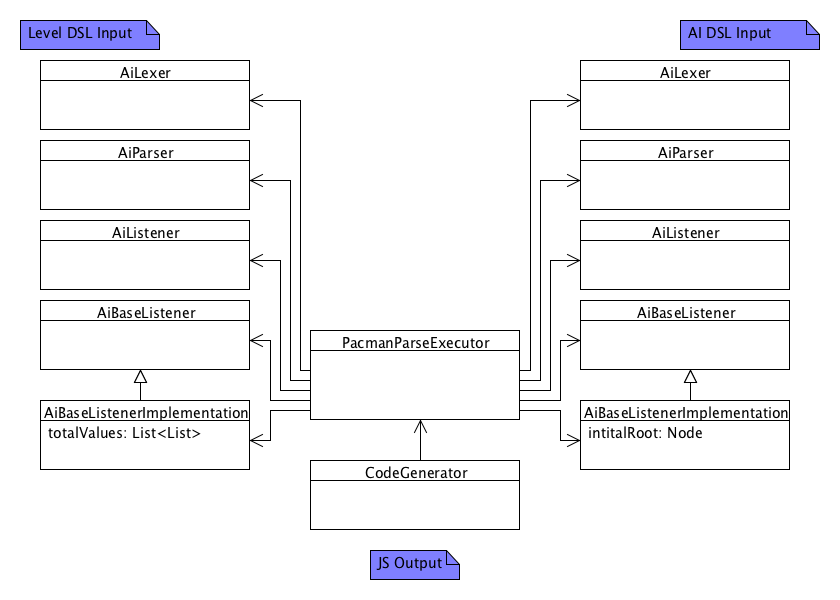
\includegraphics[width=3.3in]{code_gen_rough.png}

\caption{Beteiligte Klassen bei der Codegenerierung mit ANTLR}
\label{antlr_classes}
\end{figure}

\subsection{Level DSL}
Eine Level DSL entspricht dem CSV-Format. In der Java Klasse \texttt{LevelBaseListenerImplementation.java}, welche von LevelListener.java erbt, wird eine verschachtelte Listenstruktur erzeugt, die das Spielfeld Zeilen- und Felderweise abbildet. Die \texttt{parseLevel()} Methode, welche in der PacmanParseExecuter.java Klasse definiert ist, erwartet den Pfad zu einer .csv-Datei als Argument. Des Weiteren wird in dieser Methode die Initialisierung aller abhängigen Klassen, die für diesen Prozess nötig sind, erledigt.

Die CodeGenerator.java Klasse ist neben der Generierung für die AI auch für die Erstellung einer level.js Datei zuständig welche nach JavaScript Syntax erstellt wird. Die Datei level.js (Abbildung \ref{leveljs})
wird direkt in dem Ordner \texttt{/dsl\_pacman/pacman/levels/} generiert und von der \texttt{Gameboard}-Klasse importiert.

\begin{lstlisting}[language=Java, captionpos=b, caption=Generierte Level-Klasse in JavaScript, label=leveljs]
define([], function () {
  return {
    floor: 0,
    point: 1,
    fruit: 2,
    wall: 3,
    map: [
      [3,3,3,3,3,3,3,3,3,3,3,3,3,3,3,3,3,3,3,3],
      [3,1,1,1,1,1,1,1,1,3,1,1,1,1,1,3,1,1,2,3],
      [3,1,3,1,3,3,1,3,1,3,1,3,3,3,1,3,1,3,1,3],
      [3,1,3,1,1,1,1,1,1,1,1,1,1,3,1,3,1,3,1,3],
      [3,1,3,3,3,3,1,3,3,3,3,3,1,3,1,3,1,3,1,3],
      [3,1,1,1,1,1,1,1,1,3,1,1,1,3,1,1,1,1,1,3],
      [3,1,3,3,3,3,1,3,1,3,1,3,1,3,3,3,3,3,1,3],
      [3,1,3,3,1,1,1,1,1,2,1,1,1,1,1,1,1,3,1,3],
      [3,1,1,3,1,3,1,3,0,3,0,3,1,3,3,3,1,1,1,3],
      [3,3,1,3,2,3,1,3,0,0,0,3,1,3,2,1,1,3,1,3],
      [3,1,1,3,1,3,1,3,3,3,3,3,1,3,1,3,1,3,1,3],
      [3,1,3,3,1,1,1,1,1,1,1,1,1,3,1,3,1,3,1,3],
      [3,1,3,3,3,3,1,3,1,3,1,3,1,1,1,1,1,1,1,3],
      [3,1,1,1,1,1,1,3,1,3,1,3,1,3,3,3,3,3,1,3],
      [3,1,3,3,3,3,1,1,1,1,1,1,1,1,1,1,1,3,1,3],
      [3,1,3,1,1,1,1,3,3,3,3,3,1,3,3,3,1,1,1,3],
      [3,1,3,1,3,3,1,1,1,3,1,1,1,1,1,1,1,3,1,3],
      [3,1,3,1,3,3,1,3,1,1,1,3,3,3,3,3,3,3,1,3],
      [3,2,1,1,1,1,1,1,1,3,1,1,1,1,1,1,1,1,2,3],
      [3,3,3,3,3,3,3,3,3,3,3,3,3,3,3,3,3,3,3,3]
    ]
  }
});
\end{lstlisting}

\subsubsection{Spielfeldaufbau}
\label{spielfeldaufb}
Das Spielfeld bildet ein zweidimensionales Array ab, welches je nach Spielfeld-Design mit Zahlen von Null bis Drei befüllt wird. Die Spezifikation sieht vor, dass ein Array der Größe von exakt 20x20 erstellt werden muss. Eine beispielhafte Darstellung, die das Prinzip für den Aufbau des Spielfeldes veranschaulicht, ist in Listing \ref{gameboard_dsl} zu finden.

Zulässige Tokens sind als \emph{Value} definiert. Dies sind nur die Zahlen Null, Eins, Zwei und Drei in beliebiger Reihenfolge. Als Trennsymbol einzelner Values ist allein das Semikolon als \emph{Separator} zulässig. Diese Anreihung von Value und Trennsymbol kann beliebig oft vorkommen solange bis das Ende einer Zeile, welche als \emph{row} festgelegt ist, erreicht wird. Das Zeilenende wird durch ein \emph{LineBreak} oder aber durch ein \emph{EOF} signalisiert. Letzteres dient als terminales Symbol und signalisiert das Ende des einzulesenden Spielfeld-Arrays. Alle Zeilen zusammen bilden ein \emph{field}.


\begin{table}[!t]
%% increase table row spacing, adjust to taste
%\renewcommand{\arraystretch}{1.3}
% if using array.sty, it might be a good idea to tweak the value of
% \extrarowheight as needed to properly center the text within the cells
\caption{Spielfeld-Definition per DSL}
\label{gameboard_dsl}
\centering
%% Some packages, such as MDW tools, offer better commands for making tables
%% than the plain LaTeX2e tabular which is used here.
\begin{tabular}{|c|c|c|c|c|c|}
\hline
3 & 3 & 3 & 3 & 3\\
\hline
3 & 2 & 1 & 1 & 3\\
\hline
3 & 1 & 0 & 1 & 3\\
\hline
1 & 1 & 1 & 2 & 3\\
\hline
3 & 3 & 3 & 3 & 3\\
\hline
\end{tabular}
\begin{tabular}{|c|c|}
0 & freier Weg\\
1 & Punkt\\
2 & Frucht\\
3 & Mauer/Hindernis
\end{tabular}
\end{table}


\subsubsection{Grammatik}
Um den korrekten Aufbau des Spielfelds zu gewährleisten werden zunächst domänenspezifische Gültigkeitsregeln festgelegt. In unserem Fall sind diese durch Zahlen, Sonderzeichen und reguläre Ausdrücke repräsentiert. Die Anzahl der erlaubten Spalten ist nicht in der DSL spezifiziert. Sie wird in der \texttt{LevelListenerImplementatino} überprüft. Die im vorherigen Absatz \ref{spielfeldaufb} festgelegten Regeln werden in der Datei level.g4 (Listing \ref{level_grammar}) formal festgelegt um dann mit dem \texttt{ANTLR4} Tool Java Code zu generieren welcher zur Überprüfung der Gültigkeit des aufzubauenden Spielfeldes (Vergl. Listing\ref{leveljs}) verwendet wird.

\begin{lstlisting}[captionpos=b, caption={Auszug aus der DSL spezifizierenden Grammatik level.g4}, label=level_grammar]
grammar Level;

field: row* EOF ;
row: value (Separator value)* (LineBreak | EOF) ;

value: Value ;
Separator: ';' ;
LineBreak: '\r'?'\n' | '\r';
Value: ('0'|'1'|'2'|'3')+ ;
\end{lstlisting}

\subsection{AI DSL}
\label{ai_dsl}
Die durch Intrepretation der AI DSL generierten JavaScript-Klassen ermittelt auf Basis der aktuellen Richtung eines Geistes dessen Richtung für den folgenden Spielzug. Eingabe und Ausgabewert einer AI ist also die Richtung eines Geistes.  Aus diesem Grund ist ein Verständnis der Tokens nötig, die für das Ausdrücken einer Richtung eingesetzt werden.

\begin{table}[!t]
%% increase table row spacing, adjust to taste
%\renewcommand{\arraystretch}{1.3}
% if using array.sty, it might be a good idea to tweak the value of
% \extrarowheight as needed to properly center the text within the cells
\caption{Richtungstokens der AI DSL mit examplarischer Belegung der Tokens}
\label{ai_directions}
\centering

\begin{tabular}{|c||c||c||c||c||c||}
\hline
 \multicolumn{1}{|c||}{\bfseries Token} &  \multicolumn{1}{|c||} {\bfseries Beschreibung} &  \multicolumn{4}{|c|} {\bfseries Richtung}\\
\hline
-> & Aktuelle Richtung & R & L & U & D \\
\hline
<- & Entgegengesetzte Richtung & L & R & D & U \\
\hline
=> & Alternative Richtung & D & U & L & R \\
\hline
<= & Entgegengesetzt alternative Richtung & U & D & R & L \\
\hline
\end{tabular}
\end{table}
\label{dir_abstraction}
Tabelle \ref{ai_directions} stellt die Richtungs-Tokens dar. Hier wird durch die DSL insofern eine Abstraktion vorgenommen, als das eine Richtung relativ angegeben wird. Token \texttt{->} wird mit einem Wert aus der Menge \texttt{\{UP, DOWN, RIGHT, LEFT\}} belegt. Beim Verfassen der AI muss nicht mehr beachtet werden, welcher Richtung dieser Token bei der Ausführung des Spiels entspricht. Relevant für die Entwicklerin oder den Entwickler ist es zu entscheiden, ob ein Geist in der bisherigen Richtung weiterläuft, in eine der alternativen Richtungen ausweicht oder umkehrt.
Die entstehende Simplifizierung wird durch den Pseudocode in Listing \ref{direction_pseudo} demonstriert, der das Laufen in die entgegengesetzte Richtung ohne Abstraktionen der AI-DSL darstellt.

\begin{lstlisting}[language=Java, captionpos=b, caption=Umkehren der Richtung in Pseudocode, label=direction_pseudo]
if DIRECTION == RIGHT:
    return LEFT
elif  DIRECTION == LEFT:
    return RIGHT
elif DIRECTION == UP:
    return DOWN
elif DIRECTION == DOWN:
    return UP
\end{lstlisting}

Da die DSL die Notwendigkeit von Conditionals zur einzelnen Behandlung der Richtung entfernt, würde in Syntax der DSL ein \texttt{<-} Token genügen, um  die Logik des Pseudocodes abzubilden.
\subsubsection{Überblick der Operatoren}
\emph{Pac-Man AI DSLs} beginnen mit ihrem Namen in runden Klammern. Innerhalb dieses Blocks befinden sich Operatoren, die eine Richtung als Rückgabewert liefern. Entscheidend für das Auswählen einer Richtung ist oftmals, ob diese frei ist. Wie in Absatz \ref{umsetz} beschrieben, ist im JavaScript-Spiel der Akteur \emph{Checkmove} dafür zuständig, eine Auskunft darüber zu geben, ob eine Richtung frei ist. Die DSL bietet die in Tabelle \ref{checkmove_operators_tbl} gelisteten Operatoren an, die eine Prüfung durch Checkmove auslösen.

%\begin{lstlisting}[language=Java, captionpos=b, caption=blabla, label=amb]
\lstset{
  breaklines=true
  }

\begin{table}[!t]
%% increase table row spacing, adjust to taste
%\renewcommand{\arraystretch}{1.3}
% if using array.sty, it might be a good idea to tweak the value of
% \extrarowheight as needed to properly center the text within the cells
\caption{Operatoren mit Syntaxbeispiel, die Methode Checkmove ansteuren}
\label{checkmove_operators_tbl}
\centering
\setlength\tabcolsep{1.5pt}
\begin{tabular}{|c||l|c|l|}
\hline
& \textbf{Syntax} & \textbf{Beschreibung} & \textbf{Beispiel}\\

\hline
if* &

\begin{lstlisting}[basicstyle=\scriptsize\ttfamily]
if *(DIR) {
  //BLOCK A
} else {
 //BLOCK B
}
\end{lstlisting} &

\makecell{\textit{If-Free Operator}\\
Ausführen von A,\\
wenn Richtung DIR frei.\\
Sonst Ausführen von B.} &

\begin{lstlisting}[basicstyle=\scriptsize\ttfamily]
if *(->) {
  ->
} else {
  <-
}
\end{lstlisting} \\

\hline
** &

\begin{lstlisting}[basicstyle=\scriptsize\ttfamily]
**{
  DIR;
  DIR;
}
\end{lstlisting} &
\makecell{\textit{Filter-Free Operator}\\
Richtung die nicht\\
begehbar sind, werden entfernt.} &

\begin{lstlisting}[basicstyle=\scriptsize\ttfamily]
**{
  =>;
  <=;
}
\end{lstlisting} \\
\hline
*n &

\begin{lstlisting}[basicstyle=\scriptsize\ttfamily]
*1{
  DIR;
  DIR;
}
\end{lstlisting} &

\makecell{\textit{Filter-FreeN Operator}\\
Filter gemäß Filter-Free Operator,\\
Auswahl des n-ten Elements.} &

\begin{lstlisting}[basicstyle=\scriptsize\ttfamily]
 *1{
  =>;
  <=;
}
\end{lstlisting} \\
\hline

\end{tabular}
\end{table}

Bei den Operatoren ist zu beachten, dass die \texttt{If-Free-} und \texttt{Filter-FreeN}-Operatoren jeweils eine einzelne Richtung als Rückgabewert besitzen, wohingegen der \texttt{Filter-Free}-Operator eine Liste von Richtungen zurückgibt. Der Begriff des Rückgabewerts im Kontext der DSL bildet sich bei der Ausführung mit JavaScript Methoden ab.


Der \texttt{Filter-Free}-Operator darf beispielsweise nicht als äußerster Block einer DSL stehen, da mehrere Werte zurückgegeben werden aber nur eine einzige Richtung den Folgespielzug bestimmt. Da JavaScript eine dynamisch typisierte Sprache ist, würde ein Laufzeitfehler aufgrund eines unerwarteten Listen-Typs auftauchen. Dies ist unerwünscht, weil der Fehler spät in der Verarbeitungskette auftaucht und dessen Ursprung schwer zurückzuverfolgen ist. Eine entsprechende Validierung bei der Kompilierung der DSL wäre möglich und sinnvoll, wurde in der vorliegenden Implementierung jedoch nicht umgesetzt.

Die DSL in Listing \ref{simpledsl} benutzt den \texttt{Filter-FreeN}-Operator um die erste der übergebenen Richtungen auszuwählen, die frei ist. Erkennbar ist, dass ein Weiterlaufen in der aktuellen Richtung (\texttt{->}) vorzuziehen ist, und versucht werden soll in eine der alternativen Richtungen (\texttt{=>}, \texttt{<=}) auszuweichen, bevor umgekehrt wird (\texttt{<-}).


\begin{lstlisting}[language=Java, captionpos=b, caption=AI DSL mit F\texttt{Filter-FreeN}-Operator, label=simpledsl]
simple(
    *1{
      ->;
      =>;
      <=;
      <-;
    }
)
\end{lstlisting}

Zum zufälligen Auswählen von Richtungen führen wir den Random-Operator (Tabelle \ref{random_op}) ein.

\begin{table}[!htb]
%% increase table row spacing, adjust to taste
%\renewcommand{\arraystretch}{1.3}
% if using array.sty, it might be a good idea to tweak the value of
% \extrarowheight as needed to properly center the text within the cells
\caption{Random Operator mit Syntaxbeispiel}
\label{random_op}
\centering
\setlength\tabcolsep{1.5pt}
\begin{tabular}{|c||l|c|l|}
\hline
& \textbf{Syntax} & \textbf{Beschreibung} & \textbf{Beispiel}\\

\hline
\% &

\begin{lstlisting}[basicstyle=\scriptsize\ttfamily]
%(r:r) {
  DIR;
  DIR;
}
\end{lstlisting} &

\makecell{\textit{Random Operator}\\
Aus den Richtungen \texttt{DIR}\\ wird zufällig
ein Wert ausgewählt.\\ Die Wahrscheinlichkeit\\
ist durch den ratio-Parameter \\
\texttt{r} festgelegt.} &

\begin{lstlisting}[basicstyle=\scriptsize\ttfamily]
if *(->) {
  ->
} else {
  <-
}
\end{lstlisting} \\
\hline

\end{tabular}
\end{table}

Durch die vorgestellte Sprachmitteln lassen sich nun auch komplexere Strategien abbilden. In der DSL aus Listing \ref{if_free_dsl} ist ein \texttt{If-Free}-Block zu sehen. Ist die aktuelle Richtung des Geistes nicht frei, so wird der \texttt{else}-Block ausgewertet und mit Hilfe des \texttt{Filter-FreeN}-Operators die erste freie Richtung gemäß der gleichen Rangordnung von Listing \ref{simpledsl} gewählt. Ist die aktuelle Richtung frei, so soll mit Hilfe einer Zufallsverteilung entschieden werden, ob diese weitergegangen oder eine der freien alternativen Richtungen eingeschlagen werden soll.

\begin{lstlisting}[language=Java, captionpos=b, caption=AI DSL mit \texttt{If-Free}-Block und Zufallsverteilung, label=if_free_dsl]
random(
    if *(->) {
        %(50:25:25) {
            ->;
            **{
              =>;
              <=;
            }
        }
    } else {
      *1 {
        =>;
        <=;
        <-;
      }
    }
)
\end{lstlisting}

In Listing \ref{if_free_dsl} ist der Filter-Free Operator mit dem Random Operator geschachtelt. Die DSL erlaubt beliebige Schachtelungstiefen. Die Syntax von Listing \ref{dsl_complex_nesting} ist deshalb ebenfalls zulässig.

\begin{lstlisting}[language=Java, captionpos=b, caption=Komplexere Verschachtelung in AI DSL, label=dsl_complex_nesting]
if *(->) {
  %(50:25:25) {
    ->;
    **{
      %(50:25:25) {
        ->;
        **{
          =>;
          *1{
            <-;
            ->;
          }
          <=;
        }
    }
    =>;
    <=;
  }
}
\end{lstlisting}

\subsubsection{Aufbauen der Datenstruktur zur Codegenerierung}

Die Verschachtelung von Operatoren wird nicht \emph{direkt} durch die Grammatik definiert. Die AI-Grammatik erkennt lediglich die notwendigen Tokens (Listing \ref{ai_grammar}).

\begin{lstlisting}[language=Java, captionpos=b, caption=Ausschnitt der AI Grammatik, label=ai_grammar]
ai_body: WS* (LINE_BREAK|COMMENT|bracket_close|block_declaration||direction_statement);
bracket_open: '{';
bracket_close: '}';
block_declaration: (if_free_statement|else_free_statement|random_statement|leave_free_statement|get_nth_free_statement);
\end{lstlisting}

Die Listener Implementation baut eine Baumstruktur auf. Hierzu wird für jeden geparsten \emph{Operator} eine Klasse erstellt, die von der abstrakten Klasse \texttt{Node} erbt.


\begin{figure}[!htb]
\centering
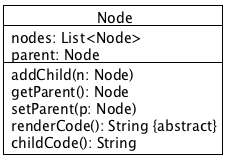
\includegraphics[width=1.7in]{node_structure_node.png}

\caption{Node-Basisklasse als Halter der Datenstruktur zu Codegenerierung}
\label{node_class}
\end{figure}

Alle Unterklassen von Node (Abbildung  \ref{node_class}) enthalten intern eine Listen-Struktur mit Kinder-Nodes. Jeder Node implementiert eine \texttt{renderCode()}-Methode, die JavaScript-Quellcode erzeugt. Der Quellcode der Kinder-Nodes wird durch Methode \texttt{childCode()} erzeugt, die über die Kinder-Nodes iteriert, jeweils \texttt{renderCode()} aufruft und die Ergebnisse als String konkateniert. Methode \texttt{childCode()} wird per Konvention in jeder Node-Klasse bei \texttt{renderCode()} aufgerufen. Eine Node-Klasse erzeugt so beim Code-Generieren ebenfalls den JavaScript-Quellcode seiner Kinder. Beim Generieren einer AI-Strategie wird \texttt{renderCode()} auf dem Wurzelknoten aufgerufen, der im Listener als Instanzvariable \texttt{initialNode} geführt ist (siehe Abbildung \ref{antlr_classes}). Abbildung \ref{node_structure_ex} zeigt die Baumstruktur zur DSL von Listing \ref{if_free_dsl}, Listing \ref{if_free_output} den generierten JavaScript-Code.


\begin{figure}[!htb]
\centering
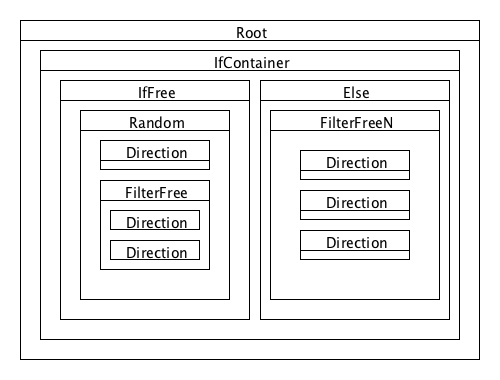
\includegraphics[width=3.5in]{node_structure_ex.png}
\caption{Schematische Darstellung der Datenstruktur beim Parsen einer AI DSL (Laufzeit).}
\label{node_structure_ex}
\end{figure}

\begin{lstlisting}[language=Java, captionpos=b, caption=Beispiel zu generiertem JavaScript-Code einer AI DSL, label=if_free_output]
 define([], function() {
    var strategy = function(queries) {
        var direction = queries.currentDirection();
        return (function() {
            if (queries.isFree(direction)) {
                return queries.randomWithDistribution([
                    50, 25, 25
                ], [
                    direction,
                    queries.filterFree([
                        queries.alternative(direction),
                        queries.alternativeOpposite(direction)
                    ])
                ]);
            } else {
                return queries.filterFreeN(1, [
                    queries.alternative(direction),
                    queries.alternativeOpposite(direction),
                    queries.opposite(direction)
                ]);
            }
        })();
    }
    return strategy;
});
\end{lstlisting}

\subsubsection{Einbindung der generierten Klassen}

Klasse \texttt{GhostQueries} dient als Mittler der generieten Strategie mit dem Ghost-Objekt. Sie ruft Methoden \texttt{currentDirection}, \texttt{gridX()}, \texttt{gridY()} und \texttt{checkMove()} auf. Der Aufruf von \texttt{checkMove()} wird von Klasse \texttt{Ghost} an \texttt{Gameboard} deligiert.
Der Aufruf der generierten Strategie mit Übergabe des Parameters GhostQueries wird in Abbildung \ref{ai_call} dargestellt.

\begin{figure}[!htb]
\centering
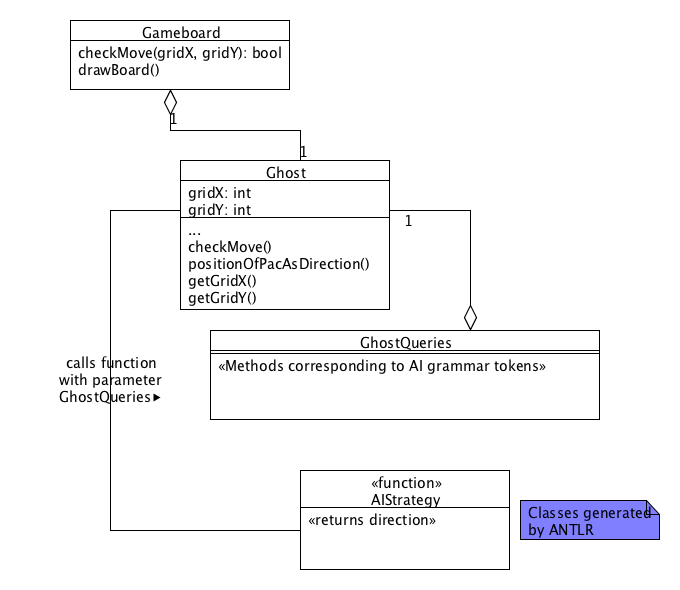
\includegraphics[width=3.3in]{queries.png}
\caption{Aufruf der generierten Strategie-Methode durch Klasse Ghost.}
\label{ai_call}
\end{figure}

Tabelle \ref{token_method_mapping} zeigt die Abbildung der Tokens der DSL auf JavaScript-Methoden der Klasse GhostQueries. In der Darstellung werden ebenfalls die Parameter- und Rückgabetypen dieser Methoden aufgeführt.


\begin{table}[!htb]
%% increase table row spacing, adjust to taste
%\renewcommand{\arraystretch}{1.3}
% if using array.sty, it might be a good idea to tweak the value of
% \extrarowheight as needed to properly center the text within the cells
\caption{Mapping von AI-Tokens auf JavaScript Methoden der Klasse \texttt{GhostQueries}}
\label{token_method_mapping}
\centering
\setlength\tabcolsep{1.5pt}
\begin{tabular}{|l||l|}

\hline
\textbf{Op} & \textbf{Methode in GhostQueries}\\

\hline
-> & currentDirection(): \emph{String} \\

\hline
<- & opposite(direction: String): \emph{String} \\

\hline
=> & alternative(direction: String): \emph{String} \\

\hline
<= & alternativeOpposite(direction: String): \emph{String} \\

\hline
if* & isFree(direction: String): \emph{Boolean} \\

\hline
** & filterFree(directions: List<String>): \emph{List<String>} \\

\hline
*n & filterFreeN(n: Number, directions: List<String>): \emph{String} \\

\hline
\% & randomWithDistribution(ratios: \emph{List<Number>}, dirs: \emph{List<String>})\\

\hline
\end{tabular}
\end{table}

\subsubsection{JavaScript-Datenstrukturen}
Neben der Abstraktion bezüglich der Richtungen (siehe Absatz \ref{dir_abstraction}) sorgt Klasse GhostQueries dafür, dass Listenstrukturen bei verschachtelten Aufrufen korrekt vereint werden. Eine Verschachtlung des \texttt{Random-Operators} mit \texttt{Filter-Free-Operator}, wie in
Abbildung \ref{node_structure_ex} gezeigt, hat zur Folge dass Parameter \emph{directions} der \texttt{randomWithDistributions()}-Methode mit einer verschachtelten Liste
befüllt wird. Die Ursache ist, dass es sich beim Ergebnis des \texttt{Filter-Free-Operator} ebenfalls um eine Liste handelt. Ein Beispiel einer entstehende Datenstruktur des directions-Parameter ist in Listing \ref{rwd_example} zu sehen.

\begin{lstlisting}[language=Java, captionpos=b, caption=Beispiel einer verschachtelten Datenstruktur als directions-Parameter von randomWithDistributions(), label=rwd_example]
[
  "UP",
  "DOWN",
  [
    "LEFT",
    "RIGHT"
  ]
]
\end{lstlisting}


Die Vereingung der Liste wird durch die underscore.js-Methode \texttt{flatten} vorgenommen. Die Idiome zur Iteration von underscore.js bestehen aus Funktionen,
die als Parameter zum einem die zu iterierende Listenstruktur übergeben bekommen und zum anderen eine Funktion die das jeweilige Listenelement
als Parameter empfängt. Für die Implementierung der Klasse GhostQueries war es sehr hilfreich, sprechende Schreibweisen wie die aus Listing \ref{underscore_speaking} einsetzen zu können. Die Syntax erinnert an moderne Programmiersprachen wie Python oder Scala, die funktionale Idiome unterstützen.

\begin{lstlisting}[language=Java, captionpos=b, caption=Implementierung der Filter-Free Methode mit Hilfe von funktionalen Hilfsmitteln von underscore.js, label=underscore_speaking]
return _.filter(_.flatten(directions), function(d) {
                return isFree(d);
            });
\end{lstlisting}

\subsubsection{Validierung}
\label{valid}

Bei der Implementierung der AI DSL hat sich bewährt, eine Baumstruktur in der entsprechende Listener-Klasse aufzubauen um diese bei der Codegeneriung zu traversieren. Hierbei taucht allerdings das Problem auf, dass \texttt{ANTLR4} keine syntaktische Validierung in Bezug auf den Aufbau dieser Baumstruktur vornimmt. Es ist also ohne manuell implementierte Validierungen nicht zu gewährleisten, dass die Operatoren der AI DSL korrekt miteinander kombiniert werden - im schlimmsten Fall resultiert ein Laufzeitfehler im JavaScipt Code.

In der Klasse \texttt{AiBaseListenerImplementation} wurde ein erster Ansatz implementiert, eine solche Validierung vorzunehmen (Listing \ref{validation_intent}). Um eine Aussagekraft für den Anwender zu haben, müsste jedoch eine präzisere Fehlermeldung mit entsprechender Zeilennummer der interpretierten DSL ausgegeben werden. Es ist abzusehen, dass der verfolgte Ansatz bei einer Erweiterung der Grammatik ungenügend ist. Hier wäre eine noch tiefere Auseinandersetzung mit \texttt{ANTLR4} empfehlenswert, um womöglich einen standartisierten Lösungsweg verfolgen zu können.

\begin{lstlisting}[language=Java, captionpos=b, caption=Grundliegende Validierung beim Hinzufügen eines einer Node in \texttt{AiBaseListenerImplementation}, label=validation_intent]

private void add(Node n) {
    if ((n instanceof Else) && !(currentNode instanceof IfContainer)) {
        System.out.println("Tried to add else without preceding if block");
    }
    if (!(n instanceof Else) && !(n instanceof IfFree) && currentNode instanceof IfContainer) {
        System.out.println("Illegal state, possible programming error: Opened an IfContainer and trying to add other than if or else block.");
    }
    this.currentNode.addChild(n);
    // Flat elements that can't contain child nodes should not set themselves as currentNode
    if (!(n instanceof Direction || n instanceof Reference || n instanceof Assignment)) {
        this.currentNode = n;
    }
}

\end{lstlisting}


\section{Fazit und Ausblick}
Ziel dieses Projekts war die Umsetzung eines funktionsfähigen Pac-Man-Klons. Ein Teil des Quellcodes sollte aus voher detailliert spezifizierten Modellen automatisch generiert werden.  Dabei wurden zwei DSLs eingesetzt. Zum einen eine DSL für die Erstellung des Spielfeldes und zum anderen eine AI DSL für die Umsetzung verschiedenen Strategien für die Bewegung der von Computer gesteuerten Figuren. Somit ist es möglich verschiedene Leveldesigns bzw. unterschiedliche Bewegungsstrategien (Erhöhung des Schwierigkeitsgrades) unabhängig vom Basiscode des Spiels zu generieren. Alle im Vorfeld gesetzten Kriterien wurden erfolgreich umgesetzt.

Ausbaubedarf besteht im Bereich der AI-DSL insbesonders bei der Validierung (siehe Abschnitt \ref{valid}). Sprechende Fehlermeldungen mit entsprechenden Zeilennummern erleichtern den Einsatz der DSL erheblich. Spezialisierte Unit-Tests für die AI DSL aufzustellen wäre ein weiterer Schritt, um die Qualität der Implementierung zu erhöhen. Eine hohe Zuverlässigkeit auf Seite der DSL Implementation sicherzustellen, wäre im realen Anwendungsfall eine Notwendigkeit.

Das Erzeugen von Code mit Hilfe von DSLs scheint in dem gegegeben Anwendungsfall in Hinblick auf Arbeitsteilung im Team äußerst sinnvoll. Es ist wahrscheinlich, dass bei einer komplexeren Pac-Man Anwendung eigenständige Teams für Level-Gestaltung und AI-Entwurf eingesetzt werden würden. Diese Teams sollten von programmiertechnischen Aspekten der eigentlichen Spiels weitesgehend entkoppelt werden um effektiv arbeiten zu können. Durch Anpassung der Codegeneratoren wären die Anwendungsentwickler in der Lage, nach Bedarf neue Technologien einsetzten zu können ohne die anderen Teams in ihrer Arbeit zu stören.


\end{document}


